% Beginning of preamble 
\documentclass[12pt]{article}  

% Useful packages for mathematical and general formatting
\usepackage{amssymb, amsmath, amsthm, amsfonts}
\usepackage{euscript}
\usepackage{graphicx}
\usepackage[dvipsnames]{xcolor}
\usepackage{url}
\usepackage{hyperref}
\hypersetup{colorlinks=true, urlcolor=RoyalBlue, citecolor=RedViolet}
\usepackage{geometry}
\geometry{left=1in, right=1in, top=1in, bottom=1in}
\usepackage{enumitem}
\usepackage{setspace} 
\setlength\parindent{0pt}
\linespread{1.2}

% Zach's Packages
\usepackage{tikz}

% Define custom environments
\newtheorem{problem}{Problem} 
\newtheorem*{theorem}{Theorem}
\newtheorem*{conjecture}{Conjecture}
\theoremstyle{definition} 
\newtheorem*{definition}{Definition}
\newtheorem*{answer}{Answer}
\newtheorem*{example}{Example}

% Font settings
\usepackage{helvet}
\renewcommand{\familydefault}{\sfdefault}

% Custom notation
\newcommand{\Z}{\mathbb{Z}}

%%%%% End of preamble %%%%%
%--------------------------------------------------------------------------

\begin{document}

\textbf{Math 3100} \hfill \textbf{Zachary Hampton} \\
\textbf{Problem Set 12} \hfill \textbf{Due Date: 12-06-2024}

\bigskip

\section*{Problem 1}

\begin{problem}
Let $A = \{a, b, c, d\}$, $B = \{a, b, c\}$, and $C = \{s, t, u, v\}$. Draw an arrow diagram of a function for each of the following descriptions. If no such function exists, briefly explain why.

\begin{enumerate}[label=(\alph*)]
    \item A function $f : A \to C$ whose range is the set $C$.
    \item A function $g : B \to C$ whose range is the set $C$.
    \item A function $g : B \to C$ that is injective.
    \item A function $j : A \to C$ that is not bijective.
\end{enumerate}
\end{problem}

\textbf{Solution:}

% Diagram for (a): A function f : A -> C whose range is the set C
\begin{center}
\textbf{Diagram for (a): $f : A \to C$ (Range = $C$)}
\newline
\newline
\begin{tikzpicture}
    % Define nodes
    \node (A1) at (0,3) {$a$};
    \node (A2) at (0,2) {$b$};
    \node (A3) at (0,1) {$c$};
    \node (A4) at (0,0) {$d$};
    
    \node (C1) at (3,3) {$s$};
    \node (C2) at (3,2) {$t$};
    \node (C3) at (3,1) {$u$};
    \node (C4) at (3,0) {$v$};
    
    % Draw arrows
    \draw[->] (A1) -- (C1);
    \draw[->] (A2) -- (C2);
    \draw[->] (A3) -- (C3);
    \draw[->] (A4) -- (C4);
\end{tikzpicture}
\end{center}

% Diagram for (b): A function g : B -> C whose range is the set C (does not exist)
\begin{center}
\textbf{Diagram for (b): $g : B \to C$ (Range = $C$) - No such function exists}
\newline
\newline
\textit{Explanation: The domain $B$ has only three elements, but $C$ has four elements. Therefore, there is no way to map all elements of $C$ (to cover its range) from $B$.}
\end{center}



% Diagram for (c): A function g : B -> C that is injective
\begin{center}
\textbf{Diagram for (c): $g : B \to C$ (Injective)}
\newline
\newline
\begin{tikzpicture}
    % Define nodes
    \node (B1) at (0,2.5) {$a$};
    \node (B2) at (0,1.5) {$b$};
    \node (B3) at (0,0.5) {$c$};
    
    \node (C1) at (3,3) {$s$};
    \node (C2) at (3,2) {$t$};
    \node (C3) at (3,1) {$u$};
    \node (C4) at (3,0) {$v$};
    
    % Draw arrows
    \draw[->] (B1) -- (C1);
    \draw[->] (B2) -- (C2);
    \draw[->] (B3) -- (C3);
\end{tikzpicture}
\end{center}

% Diagram for (d): A function j : A -> C that is not bijective
\begin{center}
\textbf{Diagram for (d): $j : A \to C$ (Not Bijective)}
\newline
\newline
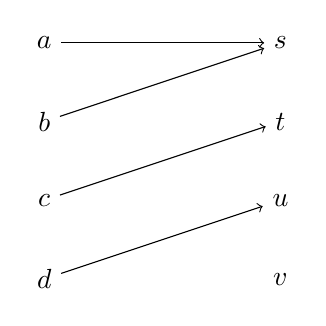
\begin{tikzpicture}
    % Define nodes
    \node (A1) at (0,3) {$a$};
    \node (A2) at (0,2) {$b$};
    \node (A3) at (0,1) {$c$};
    \node (A4) at (0,0) {$d$};
    
    \node (C1) at (3,3) {$s$};
    \node (C2) at (3,2) {$t$};
    \node (C3) at (3,1) {$u$};
    \node (C4) at (3,0) {$v$};
    
    % Draw arrows
    \draw[->] (A1) -- (C1);
    \draw[->] (A2) -- (C1); % Non-injective: a and b map to the same element
    \draw[->] (A3) -- (C2);
    \draw[->] (A4) -- (C3); % C4 (v) is not hit, so not surjective
\end{tikzpicture}
\end{center}

\newpage

\section*{Problem 2}

\begin{problem}
Determine whether each function is an injection \textbf{and} determine whether each is a surjection. You do not need formal proofs, but you must clearly justify your conclusion and show neat (and mathematically accurate) supporting work.

\begin{enumerate}[label=(\alph*)]
    \item $f : \mathbb{Z}_6 \to \mathbb{Z}_6$ defined by $f(x) = x^2 + 4 \pmod{6}$.
    \item $g : \mathbb{Z}_5 \to \mathbb{Z}_5$ defined by $g(x) = x^2 - 11 \pmod{5}$.
    \item $h : \mathbb{Z} \times \mathbb{Z} \to \mathbb{Z}$ defined by $h(x, y) = x + 2y$.
    \item $j : \mathbb{R} - \{3\} \to \mathbb{R}$ defined by $j(x) = \frac{4x}{x - 3}$.
\end{enumerate}
\end{problem}

\textbf{Solution:}

\begin{enumerate}[label=(\alph*)]
    \item In $\mathbb{Z}_6 = \{0,1,2,3,4,5\}$:
    \[
    f(0)=4, \; f(1)=5, \; f(2)=2, \; f(3)=1,\; f(4)=2,\; f(5)=5.
    \]
    Since $f(2)=f(4)$ and $f(1)=f(5)$, $f$ is not injective. The range is $\{1,2,4,5\}$, not all of $\mathbb{Z}_6$, so it is not surjective.

    \item In $\mathbb{Z}_5 = \{0,1,2,3,4\}$, note that $-11 \equiv 4 \pmod{5}$. Thus:
    \[
    g(x)=x^2+4 \pmod{5}.
    \]
    Check values:
    \[
    g(0)=4,\; g(1)=0,\; g(2)=3,\; g(3)=3,\; g(4)=0.
    \]
    Not injective since $g(1)=g(4)$ and $g(2)=g(3)$. The range is $\{0,3,4\}$, not all of $\mathbb{Z}_5$, so not surjective.

    \item Consider $h(x,y)=x+2y$ on integers. To check injectivity:
    \[
    h(0,0)=0,\quad h(2,-1)=0.
    \]
    Different inputs map to the same output, so not injective. For surjectivity, given any integer $z$, choose $x=z, y=0$, so $h(x,y)=z$. Thus $h$ is surjective.

    \item For $j(x)=\frac{4x}{x-3}$, if $j(x_1)=j(x_2)$:
    \[
    \frac{4x_1}{x_1-3}=\frac{4x_2}{x_2-3}.
    \]
    Cross-multiplying shows $x_1=x_2$. Thus $j$ is injective. For surjectivity, set $y=\frac{4x}{x-3}$. Solve for $x$:
    \[
    y(x-3)=4x \implies yx -4x =3y \implies x(y-4)=3y \implies x=\frac{3y}{y-4}.
    \]
    This works for all $y \neq 4$. When $y=4$, no solution exists. Not all real numbers are attained, so not surjective.
\end{enumerate}

\newpage

\section*{Problem 3}

\begin{problem}
Let $f : \mathbb{R} \to \mathbb{R}$ be defined by $f(x) = x^3 + 5$.

\begin{enumerate}[label=(\alph*)]
    \item Determine if $f$ is injective. If so, write a formal proof. If not, write a counterexample.
    \item Determine if $f$ is surjective. If so, write a formal proof. If not, write a counterexample.
    \item Based upon (a) and (b), is $f$ bijective?
\end{enumerate}
\end{problem}

\textbf{Solution:}

\begin{enumerate}[label=(\alph*)]
    \item \textit{Injectivity:} Suppose $f(a)=f(b)$. Then:
    \[
    a^3 + 5 = b^3 + 5 \implies a^3 = b^3 \implies a = b.
    \]
    Thus, $f$ is injective.

    \item \textit{Surjectivity:} For any $y \in \mathbb{R}$, let:
    \[
    x = \sqrt[3]{y-5}.
    \]
    Then:
    \[
    f(x) = x^3 + 5 = (y-5) + 5 = y.
    \]
    Thus, $f$ is surjective.

    \item Since $f$ is both injective and surjective, $f$ is bijective.
\end{enumerate}

\end{document}
